\documentclass[12pt]{report}
\usepackage[top=1in, bottom=1in, left=1in, right=1in, a4paper]{geometry}

 \ifx\pdftexversion\undefined
 \usepackage[dvips]{graphicx}
 \else
 
 \usepackage[pdftex]{graphicx}
 \DeclareGraphicsRule{*}{mps}{*}{}
 \fi
%\usepackage{tabularx,colortbl}
\usepackage{url}
\usepackage{chapterbib}
\usepackage{hyperref}
\usepackage{tabularx}
%\usepackage{tikz}
%\usepackage{pgfplots}
%\usepgfplotslibrary{groupplots} 
%\usepackage{pgf, pgfarrows, pgfnodes}
\usepackage{lscape}
\usepackage{longtable}
\usepackage{float}
\usepackage{url}
\usepackage{multicol}
\usepackage{color}
\usepackage{float}
\usepackage{paralist}
%\usepackage[none]{hyphenat}
\renewcommand{\bibname}{References}

\setcounter{secnumdepth}{4}
\setcounter{tocdepth}{4}

\begin{document}

\begin{titlepage}
 \begin{center}
\LARGE
\textbf{Cloud based IT Infra with Central Identity} \\
\vfill
\large
\textbf{\{ Project reboot \}}\\
\vfill
\textbf{Phase I -- Project Report }\\
\vfill
\Large
\underline{\textbf{Project Guide }} \\ 
\large
\underline{} \\
T. Chandra Shaker \\
\small
Dept. of CSE -- RGUKT Nuzvid \\
\small
\url{chandra.indra@gmail.com}
\vfill

\Large
\textbf{\underline{ Project Team } } \\
\underline{} \\
\large
\begin{tabular}{l  l}
T. Aneesh Kumar & N090247  \\
P. Nageswarao  & N091030  \\
P. Anesh  & N090977  \\
P. Jyothi Ram & N090990  \\
K. Naresh Chowdary  & N090331  \\
N. Venkata Sateesh  & N090935  \\
M. Sanyasi Rao & N090891 
\end{tabular}

\vfill



\includegraphics[width=3.5cm]{rgukt_logo.jpg} 
\Large
\underline{} \\
\underline{} \\
\normalsize
\textbf{Dept. of Computer Science and Engg. } \\
\textbf{R.G.U.K.T. - Nuzvid } \\
\textbf{Krishna Dt. - Andrha Pradesh - 521202}


\normalsize
\vfill
%\begin{multicols}{2}
%\begin{flushleft}
%\textbf{Start Date} : Sep 2014 \\
%\end{flushleft}
%
%
%\begin{flushright}
%\textbf{End Date} : Jan 2015 \\
%\end{flushright}
%\end{multicols}

\textbf{Sep 2014 -- Dec 2014 }

\end{center}
\end{titlepage}

% \pagebreak \thispagestyle{empty} \textcolor{white}{text} \pagebreak
 
\chapter*{Abstract}
\setcounter{page}{1}
\pagenumbering{roman}
\normalsize
\hspace{0.5cm} The main objective of ``Cloud based IT Infra with Central Identity'' is to utilize exisiting hardware, turn them into private clouds and access all of its services using 
Central Identity, which can be available to third party developers as API with dynamic role management and service endpoints. \newline

New private cloud based IT Infra is aimed to develop using some opensource tools like OpenStack, NFS, LDAP, Ubuntu and etc \newline

Expecting to surve with high computational virtual machines to the research, academic, learning purpose, virtual labs rather than dedicated lab hardware.

%\pagebreak \thispagestyle{empty} \textcolor{white}{text} \pagebreak

\setcounter{page}{2}
\pagenumbering{roman}
\tableofcontents
\listoffigures
\listoftables
\pagebreak \thispagestyle{empty} \pagebreak

 
\setcounter{page}{1}
\pagenumbering{arabic}


\chapter{Introduction}

\section{Introduction}
	``Cloud Based IT Infra with Central Identity'' is a complete solution, based on private cloud to enhance and effiecient utilization the IT Infrastructure of an emerging Universities and Organizations with Central Identity for all its users to access its services.\newline

	It is going to be developed in 3 phases 
	\begin{itemize}
		\item \textit{Private cloud} 
		\item \textit{Deploying Network Services} 
		\item \textit{Central Identity}
	\end{itemize}
	
\subsection{Private Cloud}

	Private Cloud establishment is targeted for hardware resource pooling, providing high computational and scalable virtual machines for deploying network based applications (smtp, proxy, ftp), web application and Network storage.
	
\subsection{Deploying Network Services}

	Configuration of Uniform hardware experience over the complete university includes single sign on on every device, configuration of mail servers etc.
	
\subsection{Central Identity}

	Essential part that combines normal network services(proxy, mail, etc.) and organizational web \& native applications. In addtion to that this central identity is available to thrid party developers as API with dynamic based role user authentication protocols.	
	

\chapter{Motivation \& Approach}

\section{Existing System}

%	We have been observing that components we are planed develop name private cloud and central identity are already exsisted but key difference here is we want to combine them and extend the central identity as Identity as a service to all emerging developers in that organization with some sort of API calls in  

\begin{itemize}
	\item The environment we observed is our university, it cosists of 7000 students and more than 500+ faculty with 6 core Engg. departments apart from 2 years of PUC course.
	\item Each Department is having strength of 700 students they arrenged these students into various various classes of 60 to 70 each, total 10 to 12 number. 
	\item Each student is provided with one Laptop with 2G RAM, 1.5GHz Clock speed and 200 GB Harddisk Storage. 
	\item All students are using these sytems for more than 8 hours in a day.
	\item All these students has to provided with course content and course labs, they are maitaining dedicated labs with 50 - 60 machines.
	
\end{itemize}


\section{Problems under consideration}

	We have observed these problems over our University
	
	\begin{itemize}
		\item Failed to maintain large user load web services  and network applications.
		\item No Central Identity, Storage \& High capacity hardware resource pool.
		%\item Redundent data in each prospect
		\item Inadequate resource requirements for Research.
		\item Dedicated computer course labs like Matlab, VLSI, etc. and these labs are useful only at lab hourse most of time they are idle.
		\item Redendent data and failed to moniter the content over student laptops.
	\end{itemize}

\pagebreak
\section{Proposed System}

	To avoid above mentioned observations we are proposing one new system with 
	\begin{itemize}
		\item Cloud based hardware resources clustering.
		\item Central Identity for Network Applicaitons with REST API.
		\item Dynamic user role management.
		\item Providing Virtual Labs (MatLab, etc.,).
		\item High Configurational Virtual Machines for research.
	\end{itemize}
	
\section{Approach}

	We want to make use of entire departmental hardaware resources more on its students laptops capacity and create a common pool of resources hence easy to maintain and moniter.\\
	
	We want to provide signle sign on implentation in each class of 60-70 laptops. such that user can use his own unique username to access university resources and later he can use the same password for network based or web based applications such as updates, mails, examinations, results etc.\newline
	
	User data can be data is retrevied from the Storage server like nfs while loging in to his laptop in any class room and his laptop's computational and storage capacity is used by the private cloud extentions that it make his laptop as slave node when ever laptop is available.\newline 
	
	User can develop application and they can use Central Identity in their application with user control and access specifations for API calls.


\chapter{System Design}
	
\section{Users \& IT Services}

	We are grouping all IT Services that are required for University into one and identifing the user who will going to use them. All Users are catagorized into 4 groups $ ^{[1]}$
	
	\begin{itemize}
	\item Studens
	\item Developers
	\item Staff, faculty
	\item Researches
	\end{itemize}
	
\begin{figure}[H]
\begin{center}
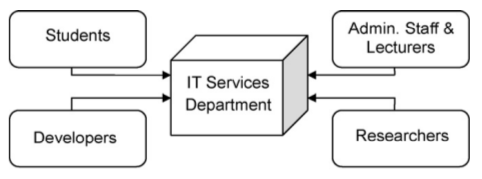
\includegraphics[width=7cm]{./it.png}
\caption{ Simplified structure of the main users of IT services in a typical university. \label{fig:Simplified structure of the main users of IT services in a typical university. }}
\end{center}
\end{figure}
	
	All University IT Services are deployed in a private cloud, constructed over exsiting infrastructure, that can be browdly viewed as 
	
\begin{figure}[H]
\begin{center}
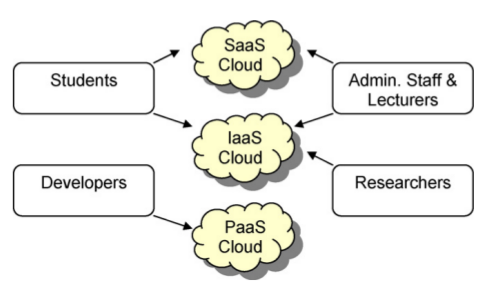
\includegraphics[width=7cm]{./it2.png}
\caption{ Simplified structure of the main users of IT services in a typical university now using the services of cloud computing\label{fig:Simplified structure of the main users of IT services in a typical university now using the services of cloud computing. }}
\end{center}
\end{figure}	
	
	
\section{Components Identified}

In this project we are restricting ourselves to some componets of the above mentioned system, we are planing to develop them in upcoming semister. We have done literature survey about these componets

\begin{itemize}
	\item Central Identiy 
	\begin{itemize}
		\item Single Sign on
		\item Identity Management
		\item Dynamic Role Based Access Control
		\item Hybrid version with REST API to third party 
	\end{itemize}
	\item Network Components
	\begin{itemize}
		\item AAA, LDAP, NFS
	\end{itemize}
	\item Cloud Infrastructure
	\begin{itemize}
		\item Cloud Computing, Private Clouds, Open Source tools 
	\end{itemize}
\end{itemize}

\chapter{Central Identiy}

\section{Single Sign-On with REST API}

\subsection{Introduction}
	Single sign on is generally a process that allows the user to access multiple 
applications requiring authentication by passing his credentials only once. The 
user first authenticates to some trusted authentication authority and then is 
granted access to all the applications trusting that authority.\\
\\
	So one of the main advantages of SSO systems is the convenience for the user. 
Another major advantage is security. There is only one place of authentication, 
which receives users credentials.Also, the user authenticates only once, so there is minimum transfer of sensitive information over the network.\\
\\
There is always a central authority, which handles user authentication. It may 
support various backend authentication mechanisms like Kerberos, LDAP, relational database, etc. The central authentication server may provide also a user interface needed to retrieve users credentials - usually a login form.\\
\\
\begin{figure}[H]
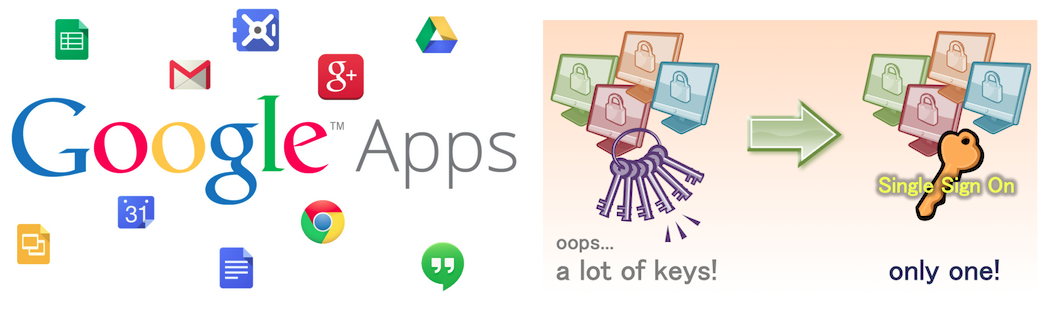
\includegraphics[width=15cm,height=5.3cm]{SSO}
\caption{Google Single Sign-On System\label{fig: Google Single Sign-On System}}
\end{figure}
\pagebreak

\subsection{Why Single Sign-On?}
\hspace{6mm}The proliferation of web applications on the Internet has led to a sharp increase in the number of accounts (and corresponding credentials) that a web user has to create and remember. Inconveniences stemming from having to keep track of the accounts, and the tendency of web sites to suffer from security breaches, in which user credentials are exposed, has resulted in a recent push to adopt single sign-on (SSO) systems more widely. As the name implies, these systems help reduce the large amount of account credentials a web user has to keep track of, by replacing these credentials with a single identity with which she can authenticate herself at many different web sites.\\
\\
\hspace{6mm}In a University scenario there exists so many applications for different purposes. And each application provides it's own sign up form for users and follow their own password policies. It would be very difficult for a user to sign up every time when a new application comes in. And storing the user information at each applications database is a waste of memory and that is a redundant process.
	\\
	\\
\hspace{6mm}By implementing Single Sign-On in the above scenarios will results in a stable \& convinient web experience for the users. And this Single Sign-On has so many advantages.
	\\
	\subsubsection{Advantages}
	\begin{itemize}
	\item Reduces the number of passwords a user has to remember and change before they expire.
	\item Reduces the risk of identity theft by limiting the number of password stored on or off campus.
	\item Users can login once and switch applications without having to login again.
	\item Allows for better audit controls and management of resource availability.
	\item Most applications/services are easier to integrate, and often can be plugged in for other services on campus.
	\item Saves time and effort of a Web Developer by providing a single button like "Login with Central Identity". No need of creating Sign Up \& Login pages for every application.
	\item Reduces phising. If users are accustomed to seeing one and only one screen when entering their credentials it may be easier for them to identify phishing attacks.
	\item Transfer of sensitive data(like User credentials) across network is minimized.
	\end{itemize}
\pagebreak
\subsection{Single Sign-On Work Flow}
Here in this section the overall workflow of Authentication in a Single Sign-On System is explained. In order to Authenticate users with the given credentials we must use a robust and stable protocol. And many Single Sign-On systems uses OAuth protocols for this purpose. Single Sign-On uses OAuth protocol for both Authentication \& Authorization.
\subsubsection{OAuth Protocol}
OAuth is an authentication protocol that allows users to approve application to act on their behalf without sharing their password.
The below figure explains the flow of Authentication in OAuth Protocol.
\begin{figure}[H]
\begin{center}
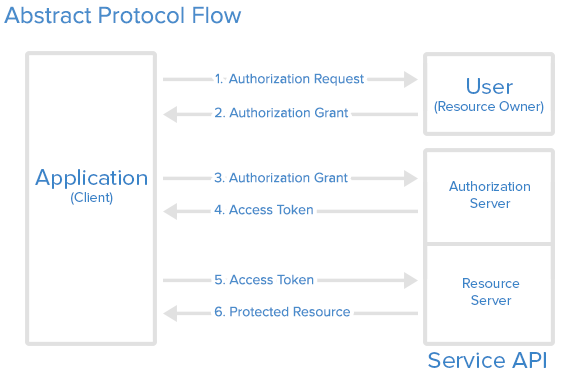
\includegraphics[scale=0.5]{abstract_flow}
\caption{OAuth Protocol Work Flow Diagram\label{fig:OAuth Protocol Work Flow Diagram}}
\end{center}
\end{figure}
Steps invloved in the above flow diagram
\begin{itemize}
\item The application requests authorization to access service resources from the user
\item If the user authorized the request, the application receives an authorization grant
\item The application requests an access token from the authorization server (API) by presenting authentication of its own identity, and the authorization grant
\item If the application identity is authenticated and the authorization grant is valid, the authorization server (API) issues an access token to the application. Authorization is complete.
\item The application requests the resource from the resource server (API) and presents the access token for authentication
\item If the access token is valid, the resource server (API) serves the resource to the application

\end{itemize}
\newpage
\section{Identity Management}
	\subsection{Introduction}
		The increasing amount of applications (web, desktop, etc.,) is one of the most important reasons why users have to remember different passwords to authenticate themselves. To simplify the use of the web applications users tend to choose the same password for every application or save the different passwords e.g., directly in the web browser. While this SSO solution is convenient for accessing the applications it also holds some security risks. For example a possible attack is phishing attack.\newline
	
             Secure Single Sign-On mechanism for web applications that were introduced in the past years can be classified in federated and user-centric identity management. Latter ones are more convenient for users as they allow them to log in with a globally unique username (e.g., their e-mail or a URL) and extended privacy by letting the user choose which personal information to send to the web applications. In referred literature they describes a solution to extended SAML-based federations with features of user-centric authentication.
   \subsection{Authentication \& Authorization}
		Due to the number and autonomy of the institutes a variety of authentication and authorization technologies are used for the different institutions. A large number of institutes use directory services (LDAP) or Kerberos, some applications use relational databases for authentication. Several legacy applications even use authentication by source IP address, which needs to be migrated in the near future. On the other hand some institutes are starting to use modern authentication techniques e.g., X.509 certificate based.\newline
   
	Traditionally identity management was done at a central point to unify authentication and authorization in heterogeneous IT infrastructures. Currently beside custom identity management there are two solutions to allow decentralized authentication and authorization in web applications: federated identity management normally SAML-based) and user-centric identity management (like OpenID).
	\subsubsection{Federated Identity Management}
		Single Sign-On was introduced on a large scale with the Kerberos protocol. For Web-based Single Sign-On OASIS issued the Security Assertion Markup Language (SAML) Standard. SAML divides the authentication and authorization in two parties (similar to Kerberos): the Service Provider (SP), being the party that holds the resources the user wants to access, and the Identity Provider (IdP), that holds the identities of the users for example at a local institute (home organization). SPs and IdPs are joined in a federation. The federation is also called an Authentication and Authorization Infrastructure (AAI). \newline
		
		Within the federation all SPs and IdPs trust each other using X.509 certificates. These certificates and addresses to resolve the handlers of the SPs and IdPs are stored in a metadata file that is distributed to all participants and builds the federation. Identity Providers issue a digitally signed assertion (or token) authenticating the user. SPs use the certificates of the IdPs published in the federation to verify the digital signature and accept the authentication. Authorization is done using attributes that the IdPs sends along with the assertion. Examples for this are Shibboleth, Liberty, and ADFS. Below figure illustrates the access to a resource protected by a Shibboleth Service Provider.
	\begin{figure}[H]
	\begin{center}
	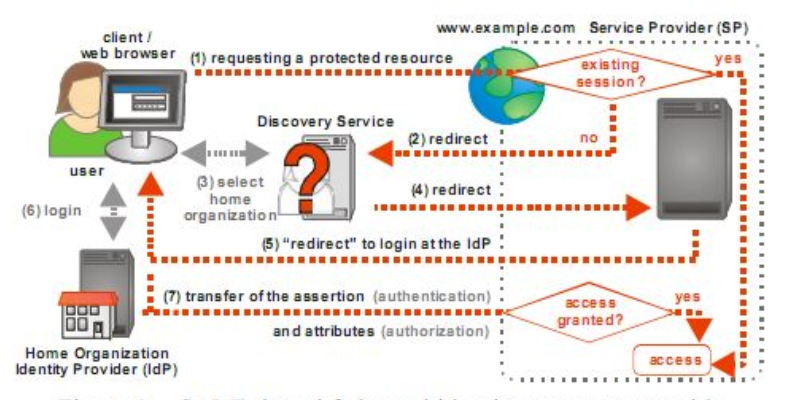
\includegraphics[width=11cm]{./3-1.png}
	\caption{ SAML based federated identity management with Shibboleth 2.0 . \label{fig:SAML based federated identity management with Shibboleth2.0. }}
	\end{center}
	\end{figure}
	Users accessing the SP are redirected to a Discovery Service (DS or WAYF server). At the DS the user selects his home organization and is redirected to his IdP that redirects him back to the SP containing the requested resource after successful authentication. A reference to the assertion issued to the user by the IdP is held as a cookie in the web browser to enable Single Sign-On. As the user subsequently accesses SPs belonging to the same federation, the browser sends the cookie referencing the assertion to the IdP and the user is directly able to access the resource without logging in again.\newline
	
	\textbf{Advantages}
	\begin{itemize}
		\item Fine grained authorization and the wide-acceptance of SAML.
		\item The SAML standard guarantees interoperability between different implementations
		\item More Secure and prevalent
	\end{itemize}
	\textbf{Dis-Advantages}
	\begin{itemize}
	\item Complexity of the protocol and user while logging
	\item Single Logout
	\item Unable to manage private info
	\end{itemize}

	\subsubsection{User-Centric Identity Management}
	The latest development in the evolution of identity management are user-centric approaches. They extends the users’ privacy as the user can decide which private information to send to the SP (Service Provider). The user presents his/her information as a card (called I-Card) to the SP. It is up to the user which card to show and what information should be on the card.\newline
	
	There is no need for a DS in this. Users can either select their I-Card to get access or log in using a globally unique identifier (e-mail or URL).  The responsible Identity Provider (IdP) can be resolved by the Service Provider (SP) using the domain of the e-mail address or the URL given by the user.
	\begin{figure}[H]
	\begin{center}
	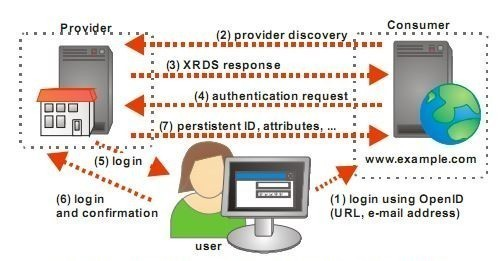
\includegraphics[width=11cm]{./3-2.jpg}
	\caption{ OpenId as an example for user-centric identity management . \label{fig:OpenId as an example for user-centric identity management . }}
	\end{center}
	\end{figure}
	Above shows an example for user-centric identity management using OpenID. Some other typical implementations are CardSpace, sxip, OAuth, Higgins. Most important extension is the ability to exchange attributes for authorization as shown for SAML.\newline
	
	\textbf{Advantages}
	\begin{itemize}
	\item Higher Usability (use of e-mail or URL)
	\item Privacy (decide which information to send to the Service Provider)
	\item Simplification of the protocol \& configuration
	\end{itemize}
	
	\textbf{Dis-Advantages}
	\begin{itemize}
	\item Security risks (like Phishing, replay attacks or web application logic flaws e.g., XSS, CSRF)
	\end{itemize}
	Besides the disadvantages because of the evolving security fixes e.g., in OpenID, user-centric solutions suffer from the fact that there is no
	single standard. Another fact that strengthens the role of OpenID is that major web companies like Google,Yahoo offer OpenID Providers for their accounts. This retention bares another disadvantage. The user has to bound to a specific Provider, if his Provider changes his terms or closes down his service, the services the user is registered for are lost.

\newpage
\section{Dynamic Role Based Access Control}

\subsection{Introduction}
	\hspace{6mm}Role Based Access Control (RBAC), also known as Non discretionary Access Control, takes more of a real world approach to structuring access control. Access under RBAC is based on a user's job function within the organization to which the computer system belongs. Essentially, RBAC assigns permissions to particular roles in an organization. Users are then assigned to that particular role.\newline
		
With the rapid development of network and the coming of information age, access control is particularly important. RBAC is an access control which is popular. RBAC authorizes and controls the roles corresponding to the users to operate the object. It solves problems of least privilege, separation of duties and so on. RBAC has better security, better flexibility, and can be well applied to the workflow system.\newline

In a role-based access control (RBAC) mechanism, these rights are defined based on the role that individuals are assigned to in an organization. It overcomes the problems in DAC (Discretionary Access Control) which is flexible but not secure and MAC (Mandatory Access Control) which is Secure but not flexible. We use roles because,\\

	\begin{itemize}
		\item Fewer relationships to manage so reduces complexity.
		\item Roles add a useful level of abstraction as organizations operate based on roles.
		\item A role is more stable than the collection of users and the collection of permissions.
	\end{itemize}

	\begin{figure}[H]
	\begin{center}
	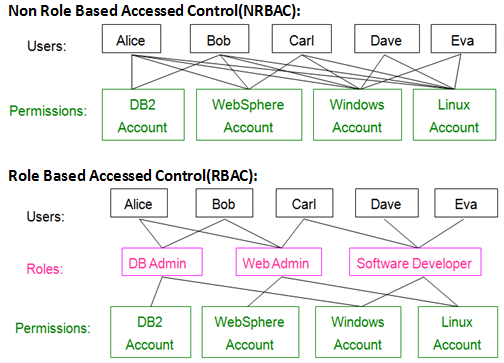
\includegraphics[width=11cm]{./4-1.png}
	\caption{ Difference between NRBAC and RBAC. \label{fig:Difference between NRBAC and RBAC. }}
	\end{center}
	\end{figure}
\newpage
	\subsection{Basic Idea of RBAC}
		Access Control policy is embodied in various components of RBAC such as 
		\begin{itemize}
		\item Role-Permission relationships
		\item User-Role relationships
		\item Role-Role relationships
		\end{itemize}
		
		 These components collectively determine whether a particular user will be allowed to access a particular piece of data in the system. RBAC components may be configured directly by the system owner or indirectly by appropriate roles as delegated by the system owner. The policy enforced in a particular system is the net result of the precise configuration of various RBAC components as directed by the system owner. The ability to modify policy to meet the changing needs of an organization is an important benefit of RBAC.
		\begin{figure}[H]
		\begin{center}
		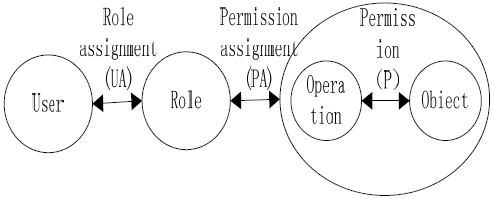
\includegraphics[width=9cm]{./4-2.png}
		\caption{ The Core Idea of RBAC. \label{fig:The Core Idea of RBAC. }}
		\end{center}
		\end{figure}
		RBAC model is defined in terms of three model components-Core RBAC, Hierarchical RBAC and Constraint RBAC. The core RBAC model includes five basic elements, i.e. U (users), R (roles), O (objects), OP (Operations) and P (permissions). The core idea of RBAC is that adds roles between users and permissions. It forms relationships among users, roles and permissions. Users get roles’ corresponding permissions by getting roles to operate on the objects.
		\begin{figure}[H]
		\begin{center}
		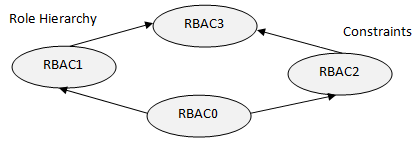
\includegraphics[width=9cm]{./4-3.png}
		\caption{ The Family of RBAC Model. \label{fig:The Family of RBAC Model. }}
		\end{center}
		\end{figure}
	\newpage	
	\subsection{Structure Diagram of  RBAC Model}
		\hspace{6mm} The Structure diagram of role based access control model consists of hierarchies and constraints. Role hierarchical relationship expresses the inheritance in roles’ permissions, such as the role A inherits role B, and then B’s permissions also belong to A. A role may inherit from multiple roles or be inherited by multiple roles. The use of role hierarchical relationship not only makes the system closer to reality, but also makes it easier to add and remove roles, easier to manage. The different types of inheritance can be,\\
		
		\begin{compactitem}
		\item User inheritance 
			\begin{itemize}
			\item means every user that is a member of r1 is also a member of r2
			\end{itemize}
			
		\item Permission inheritance
			\begin{itemize}
			\item means every permission that is authorized for r2 is also authorized r1 
			\end{itemize}					

		\item Activation inheritance 
			\begin{itemize}
			\item means that activating r1 will also activate r2
			\end{itemize}					

		\end{compactitem}
\hspace{4mm}\\
		Constraint RBAC model in RBAC adds separation of duty relations. Separation of duty can be static or dynamic. There is no formal model specified for constraints. Administrator can improve his own constraints based on requirement. Some example for constraints can be, \newline
		\begin{compactitem}
		
		
		\item Mutual Exclusion 
			\begin{itemize}
			\item No user should have more than one role in a session
			\end{itemize}
		\item Pre-condition
			\begin{itemize}
			\item Must satisfy some condition to be member of some role
			\end{itemize}					
		\item Cardinality 
		\begin{itemize}
			\item How many permission are assigning for a role
		\end{itemize}
		
		\end{compactitem}
		\begin{figure}[H]
		\begin{center}
		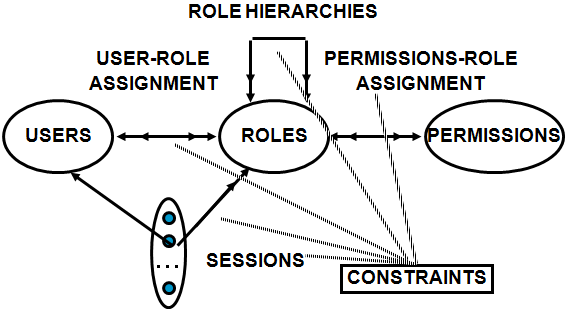
\includegraphics[width=9cm]{./4-4.png}
		\caption{ RBAC3 Model. \label{fig:RBAC3 Model. }}
		\end{center}
		\end{figure}
		\newpage
		\subsection{Dynamic Role Based Access Control Model}
		\hspace{6mm}Although RBAC has many advantages, it also has some disadvantages. it ignores the need to make dynamic constraints executed on sequential order. This problem can be solved by dynamic constraint module, so the permissions required by the sequential order can be executed by order, ensuring when the workflow occurs can operate his dynamic permission, preventing abuse of the user’s own permissions, making the system more security.\newline
		
		Dynamic RBAC overcomes the shortages of the traditional RBAC by adding with dynamic constraints and dynamic permissions, so that it makes the system easier to manage and more close to the real world. The App creator no need to go for administration, Himself, he can create roles of his own requirement. If a role is already exist, he can just add. Otherwise he can request for new roles. We can deal application depends on time.
		\begin{figure}[H]
		\begin{center}
		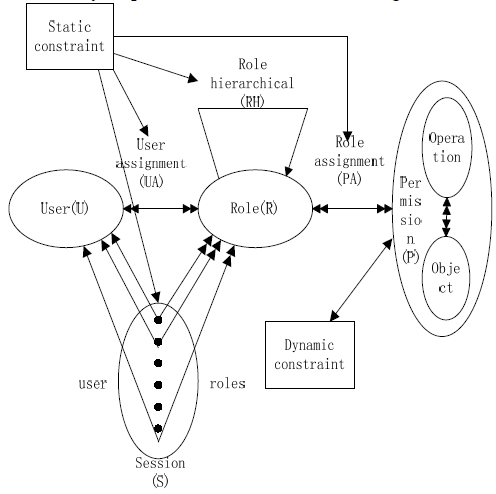
\includegraphics[width=9cm]{./4-5.png}
		\caption{ RBAC with Dynamic constraints. \label{fig:RBAC with Dynamic constraints. }}
		\end{center}
		\end{figure}
		\begin{figure}[H]
		\begin{center}
		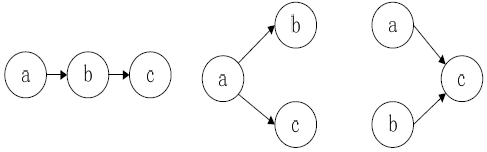
\includegraphics[width=9cm]{./4-6.png}
		\caption{ Different Types of Association. \label{fig:Different Types of Association. }}
		\end{center}
		\end{figure}

\section{Conclusion}
Federated identity management is still state of the art for Web-based Single Sign-On in scientific communities. Integration of multiple federations is a difficult task especially if usability and privacy is considered and it is very important in distributed environment. \\
\\
Single sign on helps us to assign only single key for each user for all available applications hence no redundant information about the user identification information.\\
\\
Dynamic role based access control improves security and reduces complexity by users with assigned roles and permissions to access resources of the organization.\\
\\
REST API used to connect third party developers with the orgnaizational identitiy services to their application developers and users.\\
\\
Federated central Identity with single sign on through dynamic role based access control along with the REST API for third party application developers Implementation is our main aspect.

\chapter{Network Components}

\section{Introduction}

\section{AAA}

\section{LDAP}

\section{NFS}

\section{Conclusion}

\chapter{Cloud Infrastructure}

\section{Cloud Computing}

\subsection{Introduction}

Cloud computing refers to both the applications delivered as services over the Internet and the hardware and system software in the data centers that provide those services. \\
\\
Definition -- \textit{``Cloud computing is a model for enabling convenient, on-
demand network access to a shared pool of configurable
computing resources (e.g., networks, servers, storage,
applications, and services) that can be rapidly provisioned
and released with minimal management effort or service
provider interaction''} $^{[2]}$ \\
\\
This definition includes cloud architectures, security, and deployment strategies. 

\subsection{Cloud Characterstics}
Charactersitcs of Cloud Computing can be broudly defined as \\
\\
\textit{On-demand self-service:} A consumer with an instantaneous need at a particular timeslot can avail computing resources (such as CPU time, network storage, software use, and so forth) in an automatic (i.e. convenient, self-serve) fashion without resorting to human interactions with providers of these resources.\\
\\
\textit{Broad network access:} These computing resources are delivered over the network (e.g. Internet) and used by various client applications with heterogeneous platforms (such as mobile phones, laptops, and PDAs) situated at a consumer's site.\\
\\
\textit{Resource pooling:} When we combine available resource and we can experiance accessing one super computer kind of thing is the goal of this resource pooling\\
\\
\textit{Rapid elasticity:} For consumers, computing resources become immediate rather than persistent: there are no up-front commitment and contract as they can use them to scale up whenever they want, and release them once they finish to scale down. Moreover, resources provisioning appears to be infinite to them, the consumption can rapidly rise in order to meet peak requirement at any time.\\
\\
\textit{Measured Service:} Although computing resources are pooled and shared by multiple consumers (i.e. multi-tenancy), the cloud infrastructure is able to use appropriate mechanisms to measure the usage of these resources for each individual consumer through its metering capabilities.\\
\\
\textit{Virtualization:} Virtualization is key to use the one resource or group of resource to use up to multiple instances this can be done by directly or partially

\subsection{Service Models}

If we providing any thing as a service comes, that will comes into Cloud Computing. Various Service Delivery Models listed bellow.$ ^{[3]}$

\begin{itemize}
\item Software as a Service (SaaS) -- is where in many users can make use of the software hosted by the service provider and pay only for time its being used.
\begin{itemize}
	\item Salesforce, Zoho Office and Google Apps
\end{itemize}
\item Platform as a Service (PaaS) -- provides a high-level integrated environment to design, build, test, deploy and update online custom applications.
\begin{itemize}
	\item  Google’s App Engine , Microsoft Azure and SalesForce
\end{itemize}
\item Infrastructure as a Service (IaaS) -- refers to the services provided to the users to use processing power, storage, network and other computing resources, to run any software including operating systems and applications.
\begin{itemize}
	\item  AWS, Eucalyptus, Open Stack, GoGrid and Flexiscale
\end{itemize}

\item Data storage as a Service (DaaS) -- provides data store as a service for the storage requirements of the organizations and users on the basis of pay per use model in public cloud.
\begin{itemize}
	\item   Amazon S3, DropBox, SkyDrive, etc
\end{itemize}

\item Anything as a Service (XaaS) -- is broder way of say the services in cloud computing which includes anything that is offered as a service.

\end{itemize}

\begin{figure}[H]
 \centering
 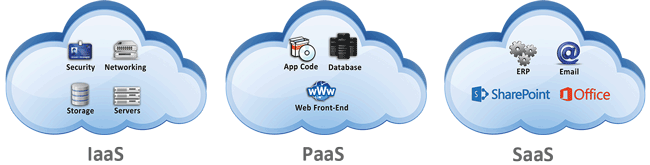
\includegraphics[width=8cm]{./service.png}
 \caption{Cloud Computing - Servcice Models \label{fig:Cloud Computing - Servcice Models} }
\end{figure}

\subsection{Deployment Models}

More recently, four cloud deployment models have been defined in the Cloud community

\begin{itemize}
\item \textit{Public cloud} -- This is the dominant form of current Cloud computing deployment model. The public cloud is used by the general public cloud consumers and the cloud service provider has the full ownership of the public cloud with its own policy, value, and profit, costing, and charging model.
\begin{itemize}
	\item   Amazon EC2, S3, Google AppEngine, and Force.com
\end{itemize}

\item\textit{ Private cloud }-- The cloud infrastructure is operated solely within a single organization, and managed by the organization or a third party regardless whether it is located premise or off premise.
\begin{itemize}
	\item   Openstack, Cloudstack, OpenNebula, Nimbus etc.
\end{itemize}
\item \textit{Hybrid cloud }-- The cloud infrastructure is a combination of two or more clouds (private, community, or public) that remain unique entities but are bound together by standardized or proprietary technology that enables data and application portability.
\begin{itemize}
	\item   Openstack APIs, AWS APIs
\end{itemize}
\item \textit{Community cloud} -- Several organizations jointly construct and share the same cloud infrastructure as well as policies, requirements, values, and concerns. The cloud community forms into a degree of economic scalability and democratic equilibrium.
\end{itemize}

\begin{figure}[H]
 \centering
 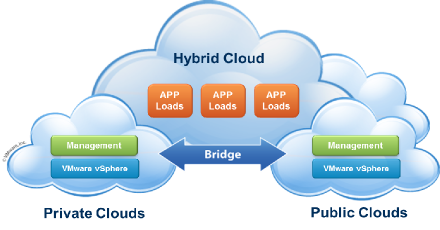
\includegraphics[width=6cm]{./model.png}
 \caption{Cloud Computing - Deployment Models \label{fig:model} }
\end{figure}


\newpage
\section{Private Clouds}

\subsection{Introduction}

\textit{Definition} -- ``It is one of the cloud deployment model where the resources of small or medium organization are united and cattered to users of the that organization or outsourced through internet'' \\
\\
The motivation to setup a private cloud within an organization has several aspects. 
\begin{itemize}
\item To maximize and optimize the utilization of existing in-house resources.
\item Security concerns including data privacy and trust also make Private Cloud an option for many firms.
\item Organizations always require full control over mission-critical activities that reside behind their firewalls.
\item Academics often build private cloud for research and teaching purposes.
\end{itemize}

\subsection{Open Source Tools}

We can construct private cloud using some open source tools like Openstack, Cloudstack, OpenNebula. \\
\\
We can use this private cloud to deploy various services like Departmental Websites, Notice Boards, Events portal, High Computational Virtual Machines for Virtual Labs, High Performance Computing, Big data analytics.
\begin{figure}[H]
 \centering
 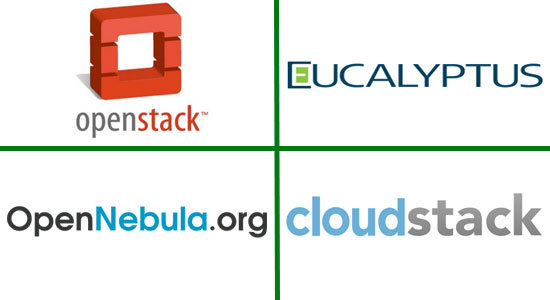
\includegraphics[width=5cm]{./cloud.jpg}
 \caption{Private Cloud - Open source tools \label{fig:cloud} }
\end{figure}

\section{Conclusion}

Hardware can be effinciently utilized by tronsforming them into cloud based infra. To maintain the institutional security we are going for privte clouds. We want to go with open source tools to maintain economically optimized.
	
\chapter{Implentation and Specifications}

\section{Implentation}

	For maintining above kind of envronment we have to setup one private cloud which will gives the highly scalable virtual machines to server the user need services on fly.\\
	
	We want to develop minal system with the above guidelines in a lab environment of 10 Master nodes and 5 client machines with uniform operating system and nfs data share. Later extended upto departmental level.
	
	
\section{Specifications}

	\begin{itemize}
		\item 15 Laptops with below configuration ( 10 Master Nodes + 5 Slave Nodes )
			\begin{itemize}
				\item 4GB RAM, 500 GB Harddisk, Intel i3 processor 1.5GHz Clock
			\end{itemize}
		
		\item Class C Network 
			\begin{itemize}
			 	\item Static IP for Master Nodes
			 	\item DHCP / Static IP for Slave Nodes
			\end{itemize}
			
		\item Uninterrupted power suply for Master Nodes.
		
	\end{itemize}
	
\section{Desired Technologies}

	\begin{itemize}
		\item Opensource private cluod tools such as Openstack, Cloudstack, etc.
		\item Ubuntu 14.04 Server LTS.
		\item LDAP Active Directories, Kerbrose, Squid for Network proxy.
		\item OAuth 2.0 with extended dynamic roles managment.
		\item Nodejs for Implementation of OAuth 2.0 as REST API.
		\item Git for Version control. 
		\item Ascii doc / python shpenix \& Latex for Documentation.
	\end{itemize}
	
\section{Expcted Results}

	We are expecting the below results after successfull implemenation of ``Cloud Based IT Infra with Central Identity'' in lab enviroment with above mentioned specifications

	\begin{itemize}	
	\item Hardware resoucre clusters from Master Nodes
	 \begin{itemize}
	 	\item 40 GB RAM
		\item 5TB of Hard disk
		\item 15 GHz Clock Speed	
	 \end{itemize}
		
	\item Hardware resoucre clusters from Slave Node (available only at active period)
	 \begin{itemize}
	 	\item 20 GB RAM
		\item 2TB of Hard disk
		\item 7.5 GHz Clock Speed	
	 \end{itemize}
	 
	\item Well Documented Implementation of Central Identity for 
	 \begin{itemize}
	 	\item Single Sign on of Client Machines.
	 	\item Network applications proxy, mails.
	 	\item University Web Services and Departmental websites.
	 	\item Third party OAuth 2.0 Implemenation as API. 
	 \end{itemize}
	\item Dynamic user role management for both Web and Native applications as API.
	\item Central Cloud Storage Pool.
	\item High Computational Virtual Machines.
	\item Virtual Labs insted of Dedicated labs in Remote Desktop or in SSH protocol.
	\item Content or Data Monitering in a Organization.
	\item Get full recovery and achieve more than 99.99\% services up time.
	\item Extendable to several departments and Universities.
	
	\end{itemize}

\chapter{References}

\section{Web References}

\begin{itemize}
\item Ubnutu OS, http://www.ubuntu.com/
\item Openstack, https://openstack.org/
\item Linux Bible, http://tuxnetworks.blogspot.com
\item OAuth 2.0, http://oauth.net/
\item Node.js https://nodejs.org
\item Git, https://github.com
\item Ascii doc, http://asciidoc.org
\item Bootstrap, http://getbootstrap.com 
\item Stack Overflow http://stackoverflow.com/

\end{itemize}
		

\end{document}